\acresetall
\chapter{Schizophrenia}
\label{ch:intro:scz}
\section*{Overview}
\Scz/ is a chronic, debilitating disease affecting approximately 1\% of the worldwide population \citep{McGrath2008}.
In the United States, it is estimated that 20\% of all \scz/ patients are homeless and \scz/ is associated with an approximately 20 year reduced life expectancy \citep{Folsom2005, Tiihonen2009}.
A 2011 World Economic Forum report \citep{Bloom2011} estimated that the global burden of mental illness -- of which \scz/ is a major contributor -- would be more than 16~trillion~US\$ over the next 20 years, or approximately 1-2\% of the 2010 global GDP per year.
Compared to all other non-communicable diseases, mental illness accounts for the most lost output, more than cardiovascular disease and cancer (\autoref{fig:intro:scz:output_loss}).
The cost of \scz/ in particular was estimated to be \$155~billion in the United States in 2013, 24\% going to direct cost of treatment, and 75\% coming from indirect costs including caregiving for patients and unemployment \citep{Cloutier2016}. 
\begin{figure}
	\centering
	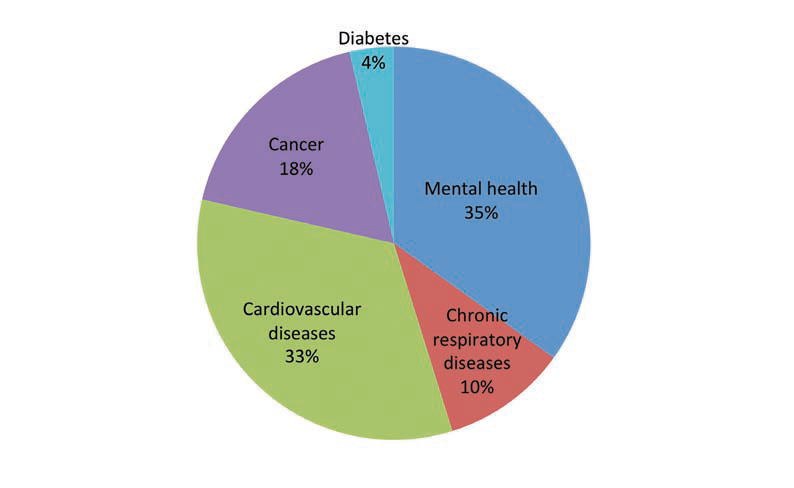
\includegraphics[width=0.7\textwidth]{intro/Bloom2011_output_loss_by_NCD}
	\caption[Breakdown of non-communicable disease cost by disease type]{Breakdown of non-communicable disease cost by disease type.
	Reproduced from \citet{Bloom2011}.}
	\label{fig:intro:scz:output_loss}
\end{figure}

\Scz/ is a syndrome defined by its symptoms, the most prominent of which is psychosis.
Symptoms are generally classified into three main categories: positive, negative, and cognitive \citep{Kay1982}.
Positive symptoms are behaviors not normally seen in healthy individuals and include hallucinations, delusions, suspiciousness, hostility, thought disorders, and movement disorders.
Negative symptoms reflect missing or disrupted normal thought processes, including: blunted affect, social withdrawal, avolition, anhedonia, and difficulty in abstract thinking.
Cognitive symptoms include attentional deficits, poor executive functioning, and both working and long-term memory impairment, specifically in the domain of episodic semantic memory.
While the positive symptoms, in particular hallucinations and delusions, might be the most prominent symptoms of \scz/, cognitive symptoms are present in up to 75\% of \scz/ patients and the severity of cognitive symptoms is strongly linked to functional outcomes \citep{O'Carroll2000, Green1996, Keefe2007}.
This is particularly troubling since treatment options for the negative and cognitive symptoms of \scz/ are extremely limited.

Since the underlying causes of \scz/ are not known, treatment for patients with \scz/ is limited to treating symptoms as they present.
Treatment for \scz/ patients primarily includes a combination of antipsychotic medication and psychosocial therapy.
Patients' responses to antipsychotics varies widely, some experiencing complete remission of psychoses and others showing no alleviation of symptoms.
Overall, following a first episode-psychosis, long-term antipsychotic treatment is effective in 30-40\% of patients in preventing future psychoses \citep{Boyer2007, Insel2010a}, leaving over half of all patients still experiencing psychotic episodes.
More importantly, antipsychotic medication only aims to treat the positive symptoms of \scz/, such as hallucinations and delusions.
There are limited treatment options for the debilitating cognitive deficits -- including deficits in attention, executive function, and both working and episodic memory -- which have proven to be the greatest barrier to rehabilitation \citep{Lieberman2005, Harrison2001, O'Carroll2000, Hyman2003}.

Like most mental disorders, the underlying etiology of \scz/ is most likely complex and heterogeneous, making the discovery of a single `monotherapy' unlikely \citep{Hyman2003}.
For these reasons, there is growing appreciation that we need to better understand and treat sets of symptoms separately, particularly developing new drug interventions for the negative and cognitive symptoms of \scz/.
Indeed, it seems likely that what today we call \scz/ is in fact a collection of related disorders, some potentially common to other mental health diagnoses as well \citep{Insel2010a}.
This view of \scz/ implies that by focusing on particular dysfunctions -- such as episodic memory impairment -- we can hope to find general therapeutic targets for diseases currently classified separately, and at the same time, by looking for convergence on to common endophenotypes we can identify treatment targets shared by patients with heterogeneous underlying etiology.
Indeed, the core unit of computation for many of these cognitive functions seems likely to be ensembles of thousands of neurons working together as a \textsc{neural circuit}.
As we have learned more about the way neural circuits govern behavior in healthy individuals, the precise nature of cognitive deficits in patients, and the molecular changes that occur in \scz/, it is becoming clear the \scz/ is at it's core a neurodevelopmental dysfunction of neural circuits \citep{Arguello2012, Insel2010a, Insel2010b, Lewis2002}.
Still, very little is known about the nature of neural circuit disruptions and how they lead to behavioral and cognitive dysfunction.

In the following sections I will expand upon some of the symptoms, brain abnormalities, and causative factors observed in \scz/ patients, with a specific focus on aspects of the disease most relevant to my main research project (see \autoref{ch:df}).
I will discuss details of the memory deficits present in \scz/ patients (\autoref{sec:intro:scz:memory}), with a particular focus on spatial and episodic memory impairments.
% I will present what we do know about underlying genetic and environmental causes of \scz/ [\ref{sec:intro:scz:genes_and_environment}], including details of 22q11.2 deletion syndrome and a mouse model of this deletion, \df/.
I will present what we know about specific brain regions affected in \scz/ patients, specifically focusing on the \ac{HPC} (\autoref{sec:intro:scz:brain}).
Finally, I will lay out several proposed causes of \scz/ including genetic risk factors, neurodevelopmental insults, alterations in neuromodulatory signaling, and disrupted glutamatergic and GABAergic machinery (\autoref{sec:intro:scz:etiology}).

\section{Memory deficits}
\label{sec:intro:scz:memory}
Disruption in working and declarative memory are among the primary cognitive deficits observed in \scz/ patients.
The memory deficits present in \scz/ are specific in that patients seem to have relatively spared implicit or procedural memory, while many patients present with striking deficits in declarative memory (see \autoref{sec:intro:memory:memory}), including both episodic memory -- conscious recollection of events -- and semantic memory -- knowledge of people, place, objects, and facts \citep{O'Carroll2000, Aleman1999, Gold2010}.
In addition to being specific, the observed memory deficits are also pervasive, in that they can not be accounted for by age, education, medication, or disease duration or severity \citep{Ranganath2008} and are present in the majority of \scz/ patients.
\todo[color=green]{cite prevalence of memory deficits in SCZ patients}
As mentioned more generally about cognitive symptoms of \scz/, the severity of memory impairments in particular is one of the strongest predictors of longterm functional outcome among \scz/ patients \citep{Green1996}, as failures in declarative memories provide the greatest barrier to steady employment.

The pattern of memory deficits observed in \scz/ patients is consistent with disruptions in both the executive control and working memory functions associated with the \ac{PFC} as well as with the longterm memory storage role of the \ac{HPC}.
Disorders that specifically arise from \ac{PFC} lesions or dysfunction show a similar impairment in encoding and retrieval as seen in \scz/ patients \citep{Ranganath2008}.
\Scz/ patients show specific impairment in working memory capacity and in the ability to work with memory held in working memory, both fundamental features of the \ac{PFC} \citep{Gold2010, Cannon2005}.
In addition, patients do not make use of the same semantic memory strategies as healthy individuals, though these impairments can at least in part be ameliorated by training or through restructuring of task stimuli -- for example, blocked instead of unblocked word lists \citep{Gold1992, Stone1998}.

\subsection{Spatial memory}
\label{sec:intro:scz:spatial}
As described in more detail above (see \nameref{sec:intro:memory:spatial-episodic}), memory for specific locations is one particular type of episodic memory that has provided tractable approaches for studying memory.
While less recognized as a core symptom of \scz/, spatial memory deficits are well documented in \scz/ patients \citep{Boyer2007, Hanlon2006, Wilkins2013, Weniger2008}, but the underlying circuit level dysfunctions have rarely been investigated \citep{Hayashi2015, Suh2013}.
A lack of general awareness of spatial memory deficits in \scz/ patients is most likely attributable to the different approaches taken by clinical psychologists and basic research scientists.
Deficits in verbal memory are among the most prominent cognitive deficits observed in \scz/ patients \citep{O'Carroll2000}.
The broad category of verbal memory reflects the nature of psychological tests used to assess memory deficits, they involve verbal discourse with the clinician.
In practice verbal memory tests generally test either short-term working memory -- with tests such as the Digit Span test which probes the number of items that one can remember and immediately recall -- or longterm declarative memory.
Longterm declarative memory tests includes remembering lists of potentially semantically grouped words or aspects of narrative stories.
This longterm declarative memory component of verbal memory tests (referred to as \textsc{secondary verbal memory}) is particularly impaired in \scz/ patients \citep{Green1996}.

In addition, the deficits observed in spatial memory seem to be specific to allocentric navigation, as compared to egocentric navigation.
For example, a study by \citeauthor{Wilkins2013} used a 4-on-8 virtual maze to distinguish between allocentric (referred to as `spatial') and egocentric (`response') navigation strategies \citep{Wilkins2013}.
The 4-on-8 virtual maze places participants in a virtual 8-arm radial maze with distal landmarks visible around the maze.
In the first phase of the task 4 arms are blocked and the participants travel to the end of the 4 open arms to receive rewards.
In the second phase all 8 arms are opened and the participants must learn to travel down the 4 newly-available arms to retrieve rewards.
Finally, in the probe trials, all 8 arms are open, with rewards in the original 4 open arms, but now the walls of the arms are raised to occlude the distal landmarks.
During these probe trials, participants who learned an egocentric strategy (e.g.~visit the 1\super{st}, 3\super{rd}, 5\super{th}, \& 6\super{th} arms clockwise around the maze) would still perform well, but those who learned an allocentric strategy (e.g.~rewards are near the mountain, forest, lake, and sun) would perform poorly.
The authors found that \scz/ patients who used an allocentric navigation strategy performed significantly worse than healthy controls, but patients who used an egocentric navigation strategy performed similar to healthy individuals.
This differential effect was also seen in learning to navigate a virtual park versus a virtual maze \citep{Weniger2008} and in a virtual Morris water maze comparing hidden- and visible-platform trials \citep{Hanlon2006}.
In agreement with the well-characterized hippocampal deficits in \scz/ patients (see \autoref{sec:intro:scz:hpc}), allocentric navigation is primarily \ac{HPC}-dependent (see \autoref{sec:intro:memory:spatial}), while egocentric navigation relies on other brain regions unaffected by \scz/, principally the caudate nucleus \citep{Hartley2003}.

Spatial memory impairments in \scz/ patients include not just deficits in allocentric spatial navigation, but in spatial working memory as well.
For example, In a similar VR radial arm maze \scz/ patients showed both working and reference memory impairments \citep{Spieker2012}.
\citeauthor{Piskulic2007} performed a meta-analysis of behavioral studies of \scz/ patients and identified consistent spatial working memory deficits in \scz/ patients \citep{Piskulic2007}.
Additionally, \ac{HPC}-\ac{PFC} synchrony is disrupted in the \df/ mouse model of \scz/ (see \autoref{sec:intro:scz:df}) during a working memory task \citep{Sigurdsson2010}.
Take together, this evidence points towards a clear fundamental disruption of spatial memory in \scz/ patients.

\section{\Scz/ in the brain}
\label{sec:intro:scz:brain}
Brain structural changes have been reliably identified in \scz/ patients following a first episode of psychosis, and more recently, in high-risk individuals during the prodrome, prior to a clinical diagnosis.
In particular, reductions in gray matter volume and a corresponding increase in lateral ventricle volume have been consistently demonstrated \citep{Fusar-Poli2013, Shepherd2012}.
% As we become aware of susceptibility genes, environmental triggers, and other prodromal markers of \scz/, the identification of an at-risk pool has allowed for the tracking of brain changes prior to the onset of psychosis.
Tracking of clinically high-risk individuals has identified \scz/-related structural changes in the hippocampal formation, the cerebellum, the superior and medial temporal lobes, the insular cortex and the \ac{PFC} \citep{Cannon2015, Millan2016}.
Additionally, among the clinically high-risk population, continued progression towards \scz/ can be predicted by monitoring gray-matter loss \citep{Tognin2014}, aiding in pre-symptomatic identification with the hope of early intervention treatments (see \nameref{sec:intro:scz:neurodevelopment}).
While there are well-characterized deficits in \scz/ patients in multiple other brain regions, including the \ac{PFC} \citep{Weinberger1986} and striatum \citep{Simpson2010}, my main research has been on hippocampal-dependent episodic memory impairment, so I will focus particularly on the \ac{HPC} in the following sections.

\subsection{The \acl{HPC} in \scz/}
\label{sec:intro:scz:hpc}
Of particular relevance to my primary thesis project, consistent behavioral, anatomical, and physiological studies of \scz/ patients have all pointed towards the \ac{HPC} as an integral region in disease pathology \citep{Boyer2007, Bogerts1985, Jakob1986}.
Meta-analysis of quantitative \ac{fMRI} studies found overall significant effect sizes of 0.37 and 0.39 for the left and right \ac{HPC} respectively, corresponding to an approximately 4\% reduction in bilateral hippocampal volume \citep{Nelson1998}.
In addition, there was no effect of illness duration, which implies that either the \ac{HPC} suddenly reduces in volume by 4\% on the day of first-episode psychosis or the hippocampal volume reduction is already present prior to clinical disease onset, further supporting the neurodevelopmental etiology of \scz/ (see \autoref{sec:intro:scz:neurodevelopment}). 
\todo[color=red, inline]{Expand on SCZ and HPC}
The medial septum projections to the \ac{HPC} are of particular interest, since the cholinergic projection has been linked to learning and memory \citep{Parent2004} and the GABAergic projection is known to target \ac{PV}+ \acp{IN} \citep{Freund1988} which are altered in \scz/ (see \autoref{sec:intro:scz:glutamate}).
In addition,  this projection has also been linked to aberrant behavior in an \ac{NMDAR} antagonist model of schizophrenia \citep{Ma2012}.
Despite these well-characterized features of hippocampal organization, it remains unknown how the function of these circuit motifs are altered in \scz/ during hippocampal-dependent behaviors.

\subsubsection{Specific role of hippocampal area CA1}
There is growing evidence that hippocampal area CA1 is the first subregion affected in \scz/, and potentially the source of hippocampal deficits.
Work by \citeauthor{Schobel2009} used high-resolution (sub-millimeter pixel size) \ac{fMRI} of baseline activity to compare \scz/ patients to healthy controls.
The authors particularly looked at regions previously associated with \scz/ (the hippocampal formation, frontal cortex, basal ganglia, and amygdala) and found a preferential increase in \ac{CBV} in \scz/ patients in hippocampal area CA1 and orbitofrontal cortex, and a decrease in dorsolateral \ac{PFC} \citep{Schobel2009}.
In addition, the authors followed a prodromal population over two years and found that baseline \ac{CBV} abnormalities specifically in hippocampal area CA1 predicted progression to psychosis.
Finally, symptom severity was also shown to correlate with \ac{CBV} levels in area CA1.
Follow-up work showed that hippocampal hypermetabolism spread from CA1 to other regions and prodromal CA1 hypermetabolism predicted post-psychosis hippocampal atrophy, and these effects are linked to deficient glutamate levels (see \autoref{sec:intro:scz:glutamate}; \citealp{Schobel2013}).
Similarly, a recent study found that progressive hippocampal area CA1 volume loss correlated with disease progression and it spread from CA1 to other hippocampal subfields \citep{Ho2017}.
In addition, the synaptic molecular machinery has been shown to be disrupted in area CA1 of \scz/ patients, with a decrease in protein levels of PSD95, synaptophysin, and scaffolding proteins \citep{Matosin2016}. 
Finally, in my primary research project (\autoref{ch:df}) I investigated the role of aberrant CA1 activity in spatial memory disruptions in a mouse model of \scz/, which further adds evidence for a central role of hippocampal area CA1 in \scz/.

\section{\Scz/ etiology}
\label{sec:intro:scz:etiology}
While the underlying cause of schizophrenia has remained elusive, and the search has been confounded by a high concordance with other psychiatric diseases \citep{Kessler2005}, collective evidence has pointed to several possible mechanistic pathways.
Unlike Alzheimer's disease or Parkinson's disease where cell-death of specific cell types has been causally linked to disease progression, \scz/ and many other psychiatric disorders exhibit no drastic cell loss or increased gliosis, and affected brain regions can span both cortical and subcortical regions, suggesting network or circuit dysfunctions \citep{Uhlhaas2012, Lewis2002}.
A clear genetic-risk component has been recognized for quite some time, which is perhaps most evident by an exponentially increasing risk for developing \scz/ with relatedness to a \scz/ patient \citep{Rodriguez-Murillo2012}.
Additional risk factors are now becoming better understood as well, including shared family environment, male gender, advanced paternal age, perinatal events, and substance abuse \citep{Lichtenstein2009}.

In my primary research project (\autoref{ch:df}) I studied a genetic mouse model of \scz/ based on a human deletion in chromosome 22 that has been strongly associated with \scz/. In the following section I will generally discuss the genetic risk structure associated with \scz/, as well as some of the best-studied molecular hypotheses of \scz/ etiology, particularly the role of dopamine and excitation-inhibition imbalance.

\subsection{Genetics}
Current estimates suggest that \scz/ is up to 80\% heritable, arising from a large network of genetic abnormalities that predispose for \scz/ \citep{Ripke2011, Tandon2008}, though most \scz/ patients do not in fact have a family history of \scz/ \citep{Tandon2008, Rodriguez-Murillo2012}.
This suggests that either \scz/ risk is conferred by many genes that individually have minimal effect, so go unnoticed unless combined with other risk factors (common disease, common allele, CDCA), or highly-penetrant individual mutations that are quickly selected against but arise \textit{de novo} leading to \scz/ (common disease-rare allele, CDRA).
Current genetic research of \scz/ focuses on three main approaches: \ac{GWA} studies, identification of \acp{CNV}, and full exome sequencing for individual mutations.

% The search for genetic risk factors has focused on several approaches, primarily genome-wide association studies (GWAS), case-studies of familial-\scz/ linked to specific highly-penetrant mutations, and newer assays for copy-number variants (CNVs) among \scz/ patients.
Linkage-based analysis has identified over 1000 proposed genes associated with \scz/, but many of these findings have failed to be replicated and their validity is questionable \citep[\url{http://www.szgene.org},][]{Allen2008}.
Large scale \ac{GWA} studies provide the ability to detect common genetic alleles which subtly contribute to \scz/ predisposition (CDCA).
A recent \ac{GWA} study of 36,989 \scz/ patients and 113,075 controls identified 108 genetic loci that reached genome-wide significance \citep{Ripke2014}.
Of the 108 loci, 83 were novel regions not previously associated with \scz/, providing new potential therapeutic targets.
Notable hits with previously recognized links to \scz/ include: the D2 dopamine receptor (\autoref{sec:intro:scz:dopamine}), glutamatergic neurotransmission (\autoref{sec:intro:scz:glutamate}), and voltage-gated calcium channels.

\acp{CNV} have been shown to confer significant risk for \scz/ and has highlighted the role of rare \textit{de novo} mutations in \scz/ \citep{Rodriguez-Murillo2012}.
Advances in sequencing technologies now allows for the sequencing of large portions of the genome of \scz/ patients, which has made possible the genome-wide unbiased search for \acp{CNV} in \scz/ \citep{Xu2011}.
A recent collaborative study of 21,094 \scz/ patients and 20,227 controls identified significantly more \acp{CNV} present in the patient population \citep{Marshall2016}, a sign of generally more genetic mutations in \scz/ patients and highlighting the link between \scz/ and \acp{CNV}.
This study specifically identified genes of synaptic function and mouse neruobehavioral phenotypes as significantly affected and in particular identified 8 loci that reached genome wide significance, including the previously identified 22q11.2, which is the basis for the genetic model that I use in my experiments and I will discuss in detail below (\autoref{sec:intro:scz:22q11}).

% These large gene chip and whole genome sequencing studies have found strong evidence for a role of \textit{de novo} \acp{CNV} as well as \ac{SNVs} in sporadic cases of \scz/ \citep{Xu2008, Xu2011}.

% Among the rare, highly penetrant mutations that have been linked to \scz/ are disruptions in the `Disrupted in schizophrenia 1' (\textit{Disc1}) gene and a large deletion at human chromosome 22q11.2.
% Disc1 was found in a Scottish family with a significantly increased prevalence of major psychiatric disorders \citep[reviewed in,][]{Brandon2009}.
% Originally associated specifically with \scz/, DISC1 is now linked with bipolar disorder and major recurrent depression as well.
% Similarly, 22q11.2 deletion syndrome leads to \scz/ in $\approx$30\% of patients, but is associated with cognitive dysfunction, bipolar disorder, and other psychiatric syndromes as well \citep{Nestler2010}.
% I worked particularly with a mouse model of 22q11.2 deletion syndrome and will expand upon this particular mutation below (\autoref{sec:intro:scz:22q11}).
% \todo[color=blue, inline]{Expand on SCZ genetics/downplay Disc1}
Sequencing the entire exomes of large populations of \scz/ patients along with healthy controls provides the opportunity to identify rare, highly-penetrant, \textit{de novo} mutations that drive \scz/ susceptibility. One such study recently identified a loss-of-function mutation in \textit{SETD1A} significantly associated with \scz/ and present in 10 of the 4,264 genomes analyzed \citep{Singh2016}.
\textit{SETD1A} is among the 3\% most constrained genes in the human genome, with no mutations found in any of the more than 9,000 matched controls, and only 2 in a separate 45,000 genome control analysis.
\textit{SETD1A} encodes an enzyme that catalyzes methylation in histone H3. Other genes in this family have also been associated with developmental disabilities and a separate \ac{GWA} study analysis identified histone modification as one of the principal pathways affected in psychiatric disorders \citep{ODushlaine2015}.

\subsubsection{Gene pathway convergence}
The genetic architecture that predisposes for \scz/ is undoubtedly complex.
To go along with recent advances in sequencing technologies that has made it possible to identify mutations in individual genes throughout the genome as mentioned above, advances in bioinformatics and a growing genetic knowledge base have allowed us to better identify the biological pathways preferentially disrupted in \scz/.
Mutations present in \scz/ patients, but not the general population, cluster within several functional domains primarily focused on signaling networks controlling neurodevelopment and synaptic transmission, particularly neuregulin and glutamate pathways (\autoref{table:intro:scz:pathways}; \citealp{Walsh2008, Glessner2010}).
Additionally, a meta-analysis combining data from \ac{GWA}, \ac{CNV}, and \ac{SNV} studies identified gene networks related to axon guidance, neuronal cell mobility, synaptic function, and chromosomal remodeling (\autoref{fig:intro:scz:cluster}; \citealp{Gilman2012}).

\begin{table}
\centering
\begin{tabular}{l c}
% \hline
\textbf{Pathway or process} & \textbf{P value} \\
\hline
Signal transduction & 0.012 \\
Neuronal activities & 0.049 \\
Nitric oxide signaling & 0.0002 \\
Synaptic long-term potentiation & 0.0005 \\
Glutamate receptor signaling & 0.003 \\
ERK/MAPK signaling & 0.004 \\
Phosphatase and tensin homolog signaling & 0.007 \\
Neuregulin signaling & 0.008 \\
Insulin-like growth factor 1 signaling & 0.008 \\
Axonal guidance signaling & 0.015 \\
Synaptic long-term depression & 0.017 \\
G protein-coupled receptor signaling & 0.034 \\
Integrin signaling & 0.036 \\
Ephrin receptor signaling & 0.042 \\
Sonic hedgehog signaling & 0.044 \\
% \hline
\end{tabular}
\caption[Pathways implicated in \scz/]{Pathways and processes overrepresented by genes disrupted in \scz/ cases. No pathways were overrepresented by genes disrupted in controls.
	Reproduced from \citet{Walsh2008}.}
\label{table:intro:scz:pathways}
\end{table}

\begin{figure}
	\centering
	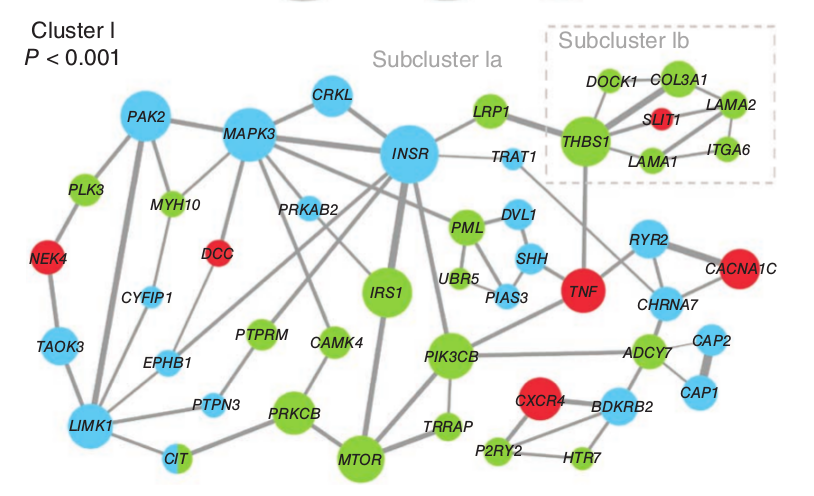
\includegraphics[width=0.9\textwidth]{intro/Gilman2012_cluster}
	\caption[First cluster identified by the NETBAG+ approach]{First cluster identified by the NETBAG+ approach.
	Cluster results from the combined set of schizophrenia-associated genetic variations: genes from \textit{de novo} \acp{CNV} are in blue, genes from non-synonymous \textit{de novo} \acp{SNV} are in light green and genes from \ac{GWA} study-implicated regions in dark red. Edge widths are proportional to the strength of the likelihood score between the two genes, and node sizes are proportional to the gene's contribution to the overall cluster score. For simplicity, only the strongest two edges from each gene are shown. Cluster I was the best cluster from the combined set of all schizophrenia genetic variations (P$<$0.001).
	Reproduced from \citet{Gilman2012}.}
	\label{fig:intro:scz:cluster}
\end{figure}

\subsection{Schizophrenia as a neurodevelopmental disorder}
\label{sec:intro:scz:neurodevelopment}
Describing \scz/ as a neurodevelopmental disorder primarily means that the pathology begins well before onset of symptoms, particularity while the brain is still developing.
The typical age for a first psychotic episode is 18-25 years, though there is evidence for pre-diagnosis symptoms from birth cohort studies, including behavioral problems, general psychopathology, intellectual and language deficits, early motor delays, poor educational performance, and stunted physical growth \citep{Welham2009}.
Additionally, prenatal (e.g.~maternal malnutrition) and perinatal (e.g.~infections) insults have shown modest links to \scz/ \citep{Lewis2002}.
It's important to distinguish the long prodromal period of \scz/ from more traditional neurodevelpomental disorders such as intellectual disability or autism.
While \scz/ disease progression may begin in early childhood, clear symptoms generally do not manifest until the second decade of life.
This time course aligns with the refinement of excitatory and inhibitory synapses associated with adolescence, so it may be that early-in-life genetic and environmental factors aren't exposed until a critical period later in life (\autoref{fig:intro:scz:neurodevelopmental}; \citealp{Insel2010a}).

\begin{figure}
	\centering
	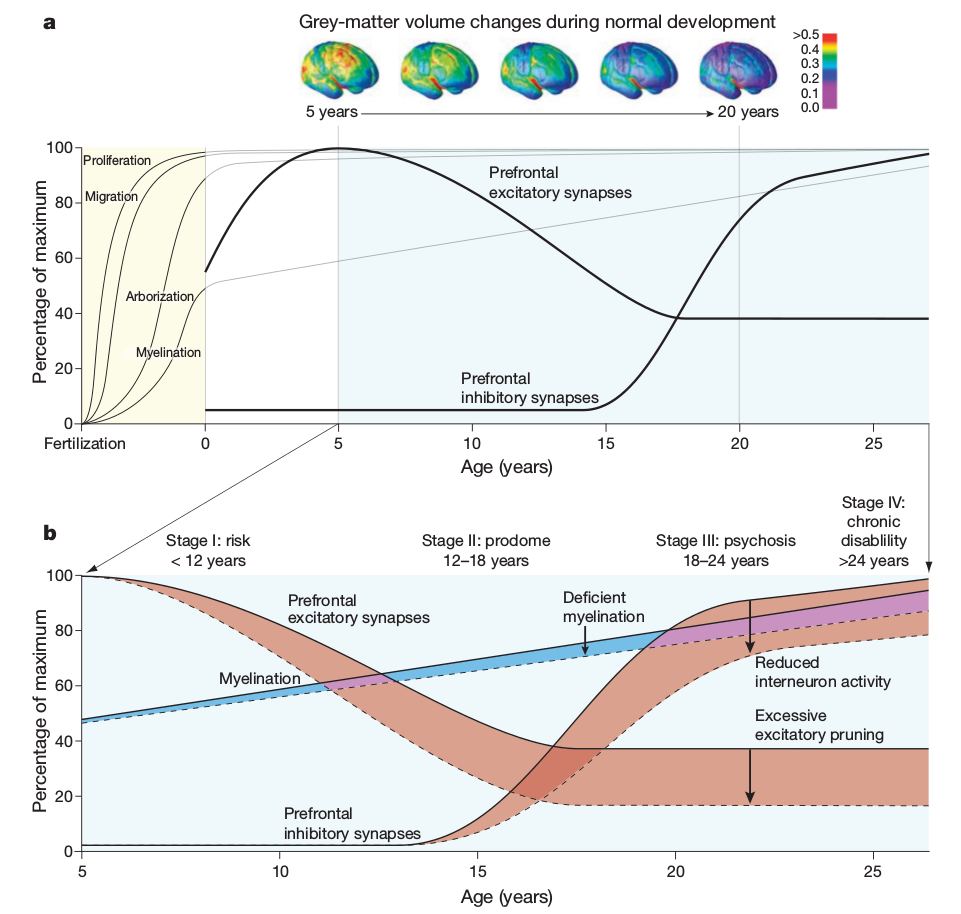
\includegraphics[width=0.9\textwidth]{intro/Insel2010_neurodevelopment}
	\caption[Neurodevelopmental model of \scz/]{Neurodevelopmental model of \scz/.
	\textbf{a}. Normal cortical development involves proliferation, migration, arborization (circuit formation) and myelination, with the first two processes occurring mostly during prenatal life and the latter two continuing through the first two post-natal decades. The combined effects of pruning of the neuronal arbor and myelin deposition are thought to account for the progressive reduction of grey-matter volume observed with longitudinal neuroimaging. Beneath this observed overall reduction, local changes are far more complex. Data from human and non-human primate brain indicate increases in inhibitory and decreases in excitatory synaptic strength occurring in prefrontal cortex throughout adolescence and early adulthood, during the period of prodrome and emergence of psychosis.
	\textbf{b}. The trajectory in children developing \scz/ could include reduced elaboration of inhibitory pathways and excessive pruning of excitatory pathways leading to altered excitatory-inhibitory balance in the prefrontal cortex. Reduced myelination would alter connectivity. Although some data support each of these possible neurodevelopmental mechanisms for schizophrenia, none has been proven to cause the syndrome. Detection of prodromal neurodevelopmental changes could permit early intervention with potential prevention or preemption of psychosis.
	Reproduced from \citet{Insel2010a}.}
	\label{fig:intro:scz:neurodevelopmental}
\end{figure}

\subsubsection{\acl{22q11.2DS}}
\label{sec:intro:scz:22q11}
Perhaps the best-established and well-studied \ac{CNV} linked to \scz/ is a deletion present in human chromosome 22 \citep[22q11.2;][]{Karayiorgou1995, Chow2006, Karayiorgou2010}.
Individuals with \ac{22q11.2DS} exhibit a spectrum of cognitive deficits as children, and $\approx$30\% of them develop \scz/ in adolescence or early adulthood, accounting for up to 2\% of all \scz/ cases \citep{Stark2008}.
Several variants of the deletion have been identified, but the critical region seems to cover 1.5 megabases including approximately 35 known genes (\autoref{fig:intro:scz:22q11_genes}).
Children with \ac{22q11.2DS} have clear cognitive impairments, reflected in a low full scale IQ, general language delays, and impairments in nonverbal, spatiotemporal and numerical tasks, in addition to general deficits in attention and working memory \citep{Karayiorgou2010}.
By early adulthood, around one third of \ac{22q11.2DS} patient are diagnosed with \scz/, making \ac{22q11.2DS} one of the highest known risk factors for developing \scz/, possibly only behind having closely related family members with \scz/ \citep{Murphy1999}.
Importantly, while \ac{22q11.2DS} is additionally associated with other psychiatric disorders through adolescence, by adulthood strict diagnoses are fairly specific for \scz/ and those who are diagnosed with \scz/ are generally indistinguishable from \scz/ patients without the 22q11.2 deletion \citep{Karayiorgou2010}.

\begin{figure}
	\centering
	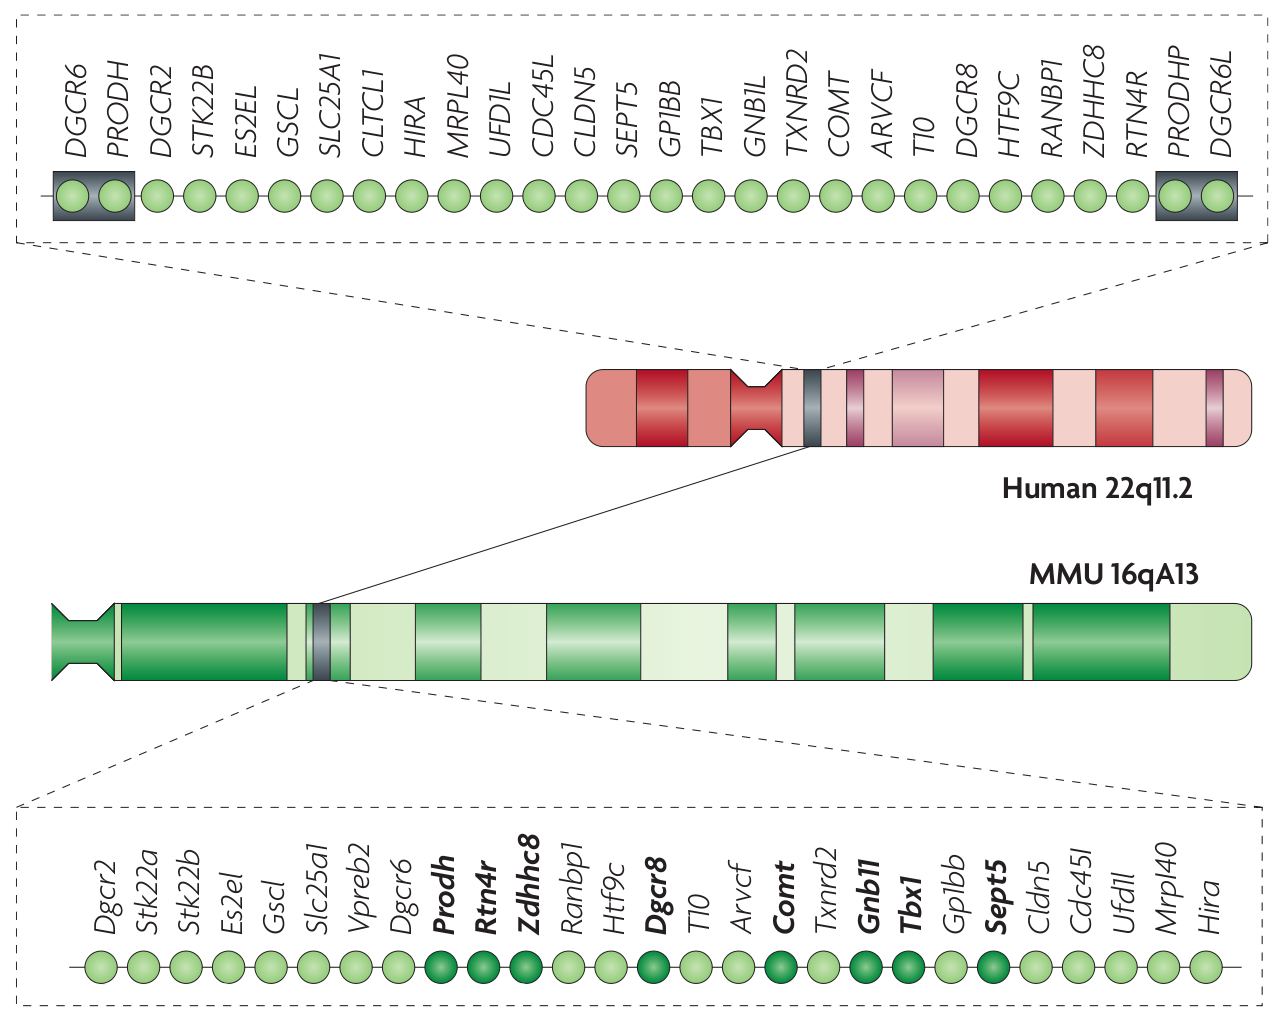
\includegraphics[width=0.8\textwidth]{intro/22q11ds_genes}
	\caption[Genetic deletion in 22q11.2DS and \df/]{Genes involved in the human 22q11.2 deletion and syntenic region in the mouse genome deleted in the \df/ mouse model. Modified from \citet{Karayiorgou2010}}
	\label{fig:intro:scz:22q11_genes}
\end{figure}

\subsubsection{\df/ mouse model of \acs{22q11.2DS}}
\label{sec:intro:scz:df}
Advances in understanding the genetic component of \scz/ predisposition have led to the development of etiologically-validated mouse models of \scz/ which will allow for the direct analysis of \textit{in vivo} neuronal network activity and identification of circuit dysfunctions present in the disease.
The homologous region to human 22q11.2 in the mouse chromosome (16qA13) is highly conserved (\autoref{fig:intro:scz:22q11_genes}), with only one gene not present in the mouse (clathrin, heavy polypeptide-like 1, CLTCL1) and one gene that is duplicated in the human region is only present as a single copy in the mouse (DiGeorge syndrome critical region 6, DGCR6p; \citealp{Karayiorgou2010}).
Several mouse models have been designed which delete various size regions from 16qA13, but I will focus on the particular model that I used in my experiments (\df/) which deletes the largest region, encompassing all of the syntenic region \citep{Stark2008}.

Behavioral tests on the \df/ mouse model have shown increased non-specific anxiety in open field and light-dark transition tasks, impaired sensorimotor gating by measuring startle response during prepulse inhibition (PPI), impaired spatial working memory in a delayed non-matching to place T-maze task, impaired working memory, and decreased freezing in a contextual fear conditioning paradigm, which could reflect either impaired contextual memory or the inability to associate the unconditioned stimuli with the context in which it was presented \citep{Drew2011b, Stark2008, Sigurdsson2010}.
Additionally, a study of immediate early gene expression using c-Fos staining following exposure to a novel environment found significantly fewer CA3 pyramidal cells active and a trend in the same direction for \acp{CA1PC} as well, which is suggestive of deficits in contextual-episodic memory, though in a direct test of spatial memory in a Morris water maze, no deficit was found \citep{Drew2011b}.
Finally, recent work in the \df/ mouse has identified a hippocampal area CA2-specific reduction in \ac{PV}+ \acp{IN}, a corresponding decrease in inhibitory activity onto CA2 pyramidal cells, and a deficit in CA2-dependent social memory \citep{Piskorowski2016}.

\textit{In vivo} neurophysiology experiments have additionally identified several deficits in this mouse model.
Experiments in hippocampal slices from \df/ mice revealed decreased inhibition of \acp{CA1PC} and induction protocol-specific deficits in Schaffer collateral \ac{LTP} \citep{Drew2011b}.
In a paper by \citeauthor{Sigurdsson2010}, the authors found that synchrony between the \ac{HPC} and \ac{PFC} was disrupted in the \df/ mouse model during a working memory task that generally relies on increased synchrony between those two brain regions and in which the \df/ mice showed a learning deficit \citep{Sigurdsson2010}.
In addition, they found that baseline synchrony predicted later task performance, suggesting a basal disruption in functional connectivity.
More recently, \citeauthor{Hamm2017} recorded neuronal activity in primary visual cortex of \df/ mice and found several indications for altered local coordination and synchrony among the neuronal population, leading to the hypothesis that disrupted local attractors lead to aberrant activity in \scz/ \citep{Hamm2017}.

Taken together, the \df/ mouse model of the human \scz/-linked \acl{22q11.2DS} effectively recapitulates cognitive deficits seen in \scz/ patients, including increased anxiety, impaired executive control, and deficits in spatial and episodic memory.
Modeling these cognitive deficits in a mouse model allows us to directly investigate underlying cellular and circuit dysfunctions.
I will discuss this topic in detail in \autoref{ch:df}, where I describe experiments studying spatial-reward memory in this etiologically-validated mouse model in order to dissect altered hippocampal circuitry in \scz/.
I will discuss the specifics later, but I found similar behavioral deficits as \citeauthor{Drew2011b}; normal baseline spatial-reward memory and deficits when faced with contextual changes, but also a robust spatial memory impairment in a task-dependent manner.

\subsubsection{Individual genes within the 22q11.2 locus}
The individual genes within the 22q11.2 locus have been characterized to varying degrees.
Mouse models of DiGeorge critical region 8 (\textit{Dgcr8}) haploinsufficiency -- a \ac{miRNA} processing gene affected by 22q11.2 deletion -- show similar working memory deficits as the \df/ mouse model of the entire 22q11.2 deletion \citep{Stark2008}.
In addition, these mice have modest alterations in \ac{PFC} neuronal morphology and increased short-term synaptic depression in mPFC layer 5 \citep{Fenelon2011}.
Suppression of a \ac{miRNA} gene within the 22q11.2 locus (\textit{miR-185}) has been shown to recapitulate some of the findings in the \df/ mouse, including simpler dendritic morphology and decreased spine density \citep{Xu2013a}.
Additionally several interventions have been successful in reversing some of these \ac{miRNA}-related abnormalities, providing potential therapies and highlighting the advantage of targeting specific molecular pathways disrupted in disease.
Repression of the downstream target of \textit{miR-185} (\textit{Mirta22}) in \df/ primary cultures reverses the structural abnormalities \citep{Xu2013a} and an activator of DGCR8 (Cobalt(III) protoporphyrin IX) can help compensate for reduced expression levels and restore \textit{miR-185} levels in mice \citep{Barr2015}.
In addition, recent work currently in press, has introduced a loss-of-function mutation in \textit{Mirta22} to the \df/ mouse, rescuing behavioral deficits (Diamantopoulou et al., in press).
Collectively these mutations implicate \ac{miRNA} processing in \scz/ disease risk and provide potential targets for therapeutic intervention.

ZDHHC8 is a palmitoyltransferase within the 22q11.2 locus that specifically targets proteins involved in axonal growth and branching.
Reintroducing ZDHHC8 in primary \df/ cultures rescues impairments in dendritic growth and synapse number, and ZDHHC8 deficiency has been shown to specifically disrupt protein localization to the axonal tip as well as disrupt AKT/GSK3$\beta$ signaling \citep{Mukai2008, Mukai2015}.

Finally, as mentioned below (\autoref{sec:intro:scz:dopamine}), dopamine misregulation seems to be a core feature of \scz/.
Two genes are present in the 22q11.2 locus related to dopamine synthesis and processing: \textit{Comt} and indirectly \textit{Prodh}.
COMT has been shown to modulate dopamine clearance in the \ac{PFC}, as extracellular dopamine clearance was 2 times slower in \textit{Comt} knockout mice \citep{Kaenmaki2010}.
PRODH is an enzyme that metabolizes \textsc{l}-proline which can modulate glutamatergic and GABAergic transmission, and has been independently linked to \scz/ \citep{Liu2002, Crabtree2016}.
\textit{Prodh}-deficient mice are hypersensitive to psychosis-inducing, dopamine-increasing amphetamine, and this is exaggerated by inhibition of COMT \citep{Paterlini2005}. 
Thus, the deletion of both of these genes in 22q11.2DS provides two `hits' which may cooperatively increase the risk of dopamine-dysfunction and \scz/.

\subsection{Dopamine}
\label{sec:intro:scz:dopamine}
The earliest mechanistic hypotheses for the disease progression of \scz/ involves disruption in normal dopamine signaling \citep{Matthysse1973}.
This hypothesis revolves around the positive symptoms of \scz/, specifically the hallucinations and delusions which can be both induced and prevented through modification of dopamine levels in the brain.
In particular, compounds that generally increase the level of dopamine (e.g.~amphetamine, LSD) lead to hallucinations similar to those experienced by \scz/ patients \citep{Angrist1994, Lieberman1987}.
Conversely, for over 60 years the primary treatment for \scz/ has been antipsychotic medications \citep{Delay1952}, which were first shown to increase the metabolism of dopamine \citep{Carlsson1963} and are now known to function primarily as D2 dopamine receptor antagonists \citep{Kapur2003}.
The general effectiveness of classical antipsychotics (e.g.~haloperidol) and the newer atypical antipsychotics (e.g.~clozapine) in treating the positive symptoms of \scz/ suggested a central role for dopamine in the more general neuropathophysiology of \scz/, but this insight has failed to expand beyond the direct treatment of psychotic episodes.
Indeed, while D2 dopamine receptor antagonists work well for many patients in managing psychotic episodes, these treatments have done very little in improving functional outcomes, as the more debilitating negative and cognitive symptoms remain untreated \citep{Insel2010a}.

The role of dopamine in \scz/ is now realized to be more nuanced than a simple consequence of a brain-wide hyperdopaminergic state.
While D2 dopamine receptor antagonist antipsychotic treatments do help manage psychotic episodes in many \scz/ patients, in some these treatments show no effect.
Additionally, post-mortem measurements of dopamine levels in \scz/ patients, as well as \textit{in vivo} measurements of dopamine activity, have not been entirely consistent across studies, and more importantly, across patients \citep{Davis1991}.
This inconsistency is most likely reflective of variability in underly disease etiology, and points to a lack of a singular disease pathology, instead suggesting a collection of underlying brain dysfunctions that funnel towards shared pathways and a commonly identified set of expressed symptoms.

% Dopamine and salience
\todo[inline, color=yellow]{SCZ as a salience disorder, role of DA}

\todo[color=cyan, inline]{section on role of hippocampal DA dysfunction in the SCZ could be added (The hippocampal-VTA loop: controlling the entry of information into long-term memory. Lisman JE, Grace AA)}
\todo[color=cyan, inline]{Add a chapter on Dopamine in limbic system -- maybe before the striatum -- and the dopamine VTA model of SCZ  - Lisman review and model. It is relevant and balances out the striatum part here. }

\subsubsection{Dopamine in the striatum}
% \citep{Bogerts1985}
One brain region in particular, the striatum, has been identified as a potential target for altered dopamine signaling.
Using radiolabeled L-dopa, presynaptic dopamine levels have been consistently shown to be elevated in the striatum of \scz/ patients \citep[reviewed in][]{Howes2007}.
At the same time, also in the striatum, D2/3 dopamine receptors (the primary receptor subtypes in this brain region) are modestly (10-20\%) elevated, independent of treatment with antipsychotic drugs \citep[reviewed in][]{Howes2009}.
% In contrast to the striatum, D1 dopamine receptors predominantly mediate dopamine activity, and while the effect is not as consistent, receptor levels show an association with severity of cognitive and negative symptoms in \scz/ \citep{Goldman-Rakic2004}.
Studies have also found evidence for increased dopamine uptake in the striatum, and post-mortem studies have found elevated dopamine and dopamine metabolite levels in the striatum \citep{Simpson2010}.
In addition, post-mortem studies have reported increased levels of striatal dopamine D2 receptors in un-medicated human patients compared to unaffected controls, suggesting a possible source of dopamine mis-regulation \citep{Cross1981}.

In order to study this potential \scz/ pathway, \citeauthor{Kellendonk2006} characterized a striatal dopamine hyper-activity mouse model that over-expresses the dopamine D2 receptor (D2R-OE) specifically in the striatum \citep{Kellendonk2006}.
They showed that increased D2 dopaimine receptor activity in the striatum leads to deficits in \ac{PFC}-dependent working-memory tasks and an increased dopamine-induced excitability in \ac{PFC} cells.
The mesolimbic pathway is a potential mechanism of action, where striatal \acp{MSN} have altered excitability due to over-expression of D2 dopamine receptors which then project to the \ac{VTA} dopaminergic neurons, which in turn project to the \ac{PFC}, which feeds back on to striatal \acp{MSN}.
Recent work has shown that both the tonic and burst firing rates of \ac{VTA} neurons are altered in the D2R-OE mouse model, though neurons in the \acl{SN} are unaffected, despite both being dopaminergic centers that receive strong projections from the striatum \citep{Krabbe2015}.


% D2r presynaptic striatum
% hypodopamine frontal?
% dopamine spcific to psychoses
% many underlying causes that converge on dopamine (complex genetic interactions and environmental hits)
% subcortical hyperdopaminergia, prefrontal hypodopaminergia

\subsection{Excitation and inhibition}
\label{sec:intro:scz:glutamate}
It has additionally been proposed that an imbalance in the levels of excitatory and inhibitory activity during development underlies \scz/ \citep{Insel2010a, Coyle2006, Yizhar2011}.
Similar to how the effectiveness of D2 dopamine-receptor targeting antipsychotics gave rise to the `dopamine hypothesis' of \scz/, one of the main pieces of evidence in support of a `glutamate hypothesis' of \scz/ etiology is the effect of \ac{NMDAR} modulators in \scz/ patients.
\ac{NMDAR} antagonists, such as phencyclidine and ketamine, induce psychoses in healthy subjects reminiscent of hallucinations observed in \scz/ patients \citep{Javitt1991, Krystal1994} and have also been shown to cause similar spatial memory deficits as in \scz/ patients along with corresponding aberrant activity in the \ac{HPC} \citep{Morgan2014}.
\Scz/ patients are also particularly sensitive to the effect of these drugs, as they worsen psychotic events.
In addition, \ac{NMDAR} antagonists induce \scz/-like symptoms in mice \citep{Inta2010}.
Finally, despite poor blood-brain barrier penetrance, \ac{NMDAR} agonists significantly improve negative symptoms in \scz/ patients.
Specifically, drugs targeting the \ac{NMDAR} glycine binding site show potential to alleviate symptoms \citep{Tsai1998, Coyle2012}.

Postmortem analysis has found mixed, and generally not robust, changes in \ac{NMDAR} levels in \scz/ patients relative to healthy controls, but increased levels of \ac{NMDAR} antagonists does seem to be consistent.
In particular, reduced glutamate and reduced catabolism of an endogenous \ac{NMDAR} antagonist (N-acetylaspartylglutamate) was found selectively in the \ac{HPC} and \ac{PFC} \citep{Tsai1995}. 
% \todo[color=cyan, inline]{Start a new par here for interneurons. Expand this chapter more on PV disfunction in CA1 and the recent CA2 reults -- make sure you include the Piskorowski paper from Siegelbaum. Steve is really into these studies now and i am sure he wants to see it here with some more background and he will riase this as a general question during the defense.}
Also, postmortem studies have found decreased levels of pre-synaptic GABAergic machinery, including GAT, GAD67, and \ac{PV}, in both the \ac{PFC} and HPC \citep{Coyle2006, Zhang2002, Konradi2011}.
In particular, \scz/ patient have shown decreased levels of \ac{PV} leading to hypofunction of \ac{PV}+ \acp{IN} in the \ac{PFC} as well as decreased numbers of \ac{PV}+ \acp{IN} in the HPC \citep{Zhang2002, Lewis2005}, especially in area CA2 \citep{Knable2004}.
Recent work from \citeauthor{Piskorowski2016} has shown that reduction in \ac{PV}+ \acp{IN} in area CA2 of the \df/ mouse has profound effects on pyramidal cell excitability and disrupts CA2-dependent social memory \citep{Piskorowski2016}.
In agreement with the well-established memory deficits present in \scz/ patients (see \autoref{sec:intro:scz:memory}), \ac{PV}+ \acp{IN} are also especially important for normal memory processing \citep{Korotkova2010, Murray2011, Donato2013}.
One possible link between these excitatory and inhibitory pathways was identified by \citeauthor{Grunze1996},  who showed that GABAergic \acp{IN} in hippocampal area CA1 are 10~times more sensitive to \ac{NMDAR}-antagonist than pyramidal cells, and thus elevated \ac{NMDAR}-antagonists levels would have a disynaptic disinhibitory effect on pyramidal cells leading to disrupted pattern recognition \citep{Grunze1996}.
Despite this significant histological evidence, there is currently limited data available on how the \textit{in vivo} activity of hippocampal GABAergic \acp{IN} is altered in \scz/.

\section{Summary}
\Scz/ is a devastating disorder of psychoses and cognitive deficits.
Hallucinations and psychoses are treatable to varying degrees of success, leaving the cognitive deficits as the least treatable and largest barrier to functional recovery.
Episodic memory impairment is a core component of the cognitive deficits in \scz/.
The \acl{HPC} is necessary for normal episodic memory in healthy individuals and is consistently identified as being altered in \scz/ patients.
By making use of a genetic mouse model of \scz/ (\df/) made possible by the growing understanding of the network of genetic mutations predisposing for \scz/, I will show specific functional correlates of impaired hippocampal activity during an episodic memory task that I identified in my primary thesis project (\autoref{ch:df}).